\documentclass{beamer}
\usepackage{amsmath}
\usepackage{icomma}
\usepackage[utf8]{inputenc}
\usepackage[T1]{fontenc}
\usepackage{polski}
\usepackage[polish]{babel}
\usepackage{hyperref}
\usepackage{float}
\usepackage{textcomp}
\usetheme{Darmstadt}
\usecolortheme{rose}

% Naprawa nazw z angielskiego
\def\figureautorefname{Rysunek}

%Strona streszczenia
\newenvironment{abstractpage}
  {\cleardoublepage\vspace*{\fill}\thispagestyle{empty}}
  {\vfill\cleardoublepage}
  
%Samo streszczenie
\newenvironment{abstractsection}[1]
  {\bigskip\selectlanguage{#1}%
   \begin{center}\bfseries\abstractname\end{center}}
  {\par\bigskip}

%Ładne ułamki w jednostkach fizycznych
\sisetup{per-mode=symbol}%

\beamertemplatenavigationsymbolsempty
\setbeamertemplate{footline}[frame number]

\begin{document}
	\section{Wprowadzenie}
	\begin{frame}
		\title[Omnivelma]{Symulacja dookólnej bazy mobilnej}
		\author{Radosław Świątkiewicz}
		\date{\today}
		\institute{Wydział Elektroniki i Technik Informacyjnych \\ Politechnika Warszawska}
		\titlepage
	\end{frame}
	\begin{frame}
		\frametitle{Spis treści}
		\tableofcontents[currentsection]
	\end{frame}
	\begin{frame}
		\begin{description}
			\item[Autor] Radosław Świątkiewicz
			\item[Promotor] dr hab. inż. Wojciech Szynkiewicz \\ Zespół Programowania Robotów i Systemów Rozpoznających \\ Instytut Automatyki i Informatyki Stosowanej
			\item[Projekt] \url{https://github.com/Antyradek/omnivelma}
		\end{description}
	\end{frame}
	
	\section{Cel}
	\begin{frame}
		\frametitle{Co kryje się w P109}
		\begin{columns}[c]
			\column{0.5\textwidth}
			\centering
			\includegraphics[width=0.8\textwidth]{graphics/velma.png} \\
			Robot manipulacyjny Velma
			\column{0.5\textwidth}
			\centering
			\includegraphics[width=\textwidth]{graphics/omnivelma.png} \\
			Platforma na kołach Mecanum
		\end{columns}
	\end{frame}
	\begin{frame}
		\frametitle{Co to jest model}
		Po co potrzebny jest model:
		\begin{itemize}
		 \item Pozwala bezpiecznie testować nowe oprogramowanie.
		 \item Przyspiesza budowanie algorytmów sterowania.
		 \item Ułatwia przeprowadzanie skomplikowanych testów.
		 \item Daje możliwość implementacji nieistniejących czujników.
		\end{itemize}
		Wymagania:
		\begin{itemize}
		 \item Reaguje na siły w podobny sposób, co robot.
		 \item Przyjmuje takie samo sterowanie.
		 \item Generuje odpowiednie dane z wirtualnych czujników.
		\end{itemize}
	\end{frame}
	
	\section{Platforma}
	\begin{frame}
		\frametitle{Koła Szwedzkie (Mecanum)}
		\centering
		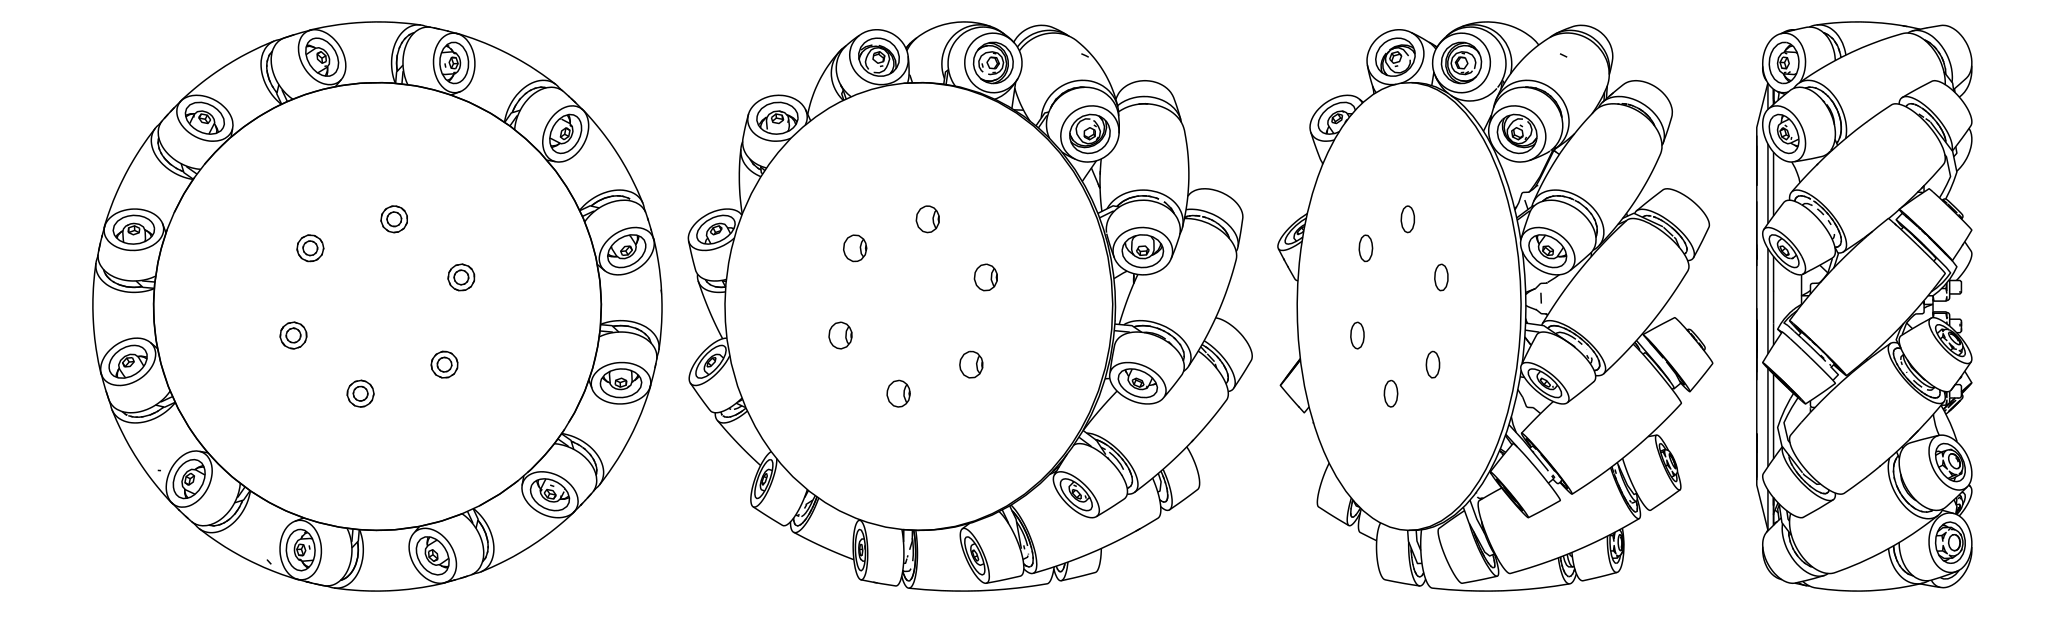
\includegraphics[width=\textwidth]{graphics/wheel.pdf}
		\begin{itemize}
			\item Pozwalają na dowolny obrót i ruch pojazdu w każdą stronę.
			\item Rolka obrócona względem osi o 45\textdegree.
			\item Każde koło ma 12 pasywnych rolek.
			\item Punkt kontaktu powinien płynnie przechodzić z rolki na rolkę.
		\end{itemize}
	\end{frame}
	\begin{frame}
		\frametitle{Podobne koła}
		\begin{columns}[c]
			\column{0.5\textwidth}
			\centering
			\includegraphics[width=\textwidth]{graphics/omni.png} \\
			Koło wielokierunkowe.\footnotemark[2]
			\column{0.5\textwidth}
			\centering
			\includegraphics[width=\textwidth]{graphics/heavy.png} \\
			Bardziej wytrzymałe koło.\footnotemark[3]
		\end{columns}
	\footnotetext[2]{http://www.robotshop.com}
	\footnotetext[3]{“Mechanical development of an automated guided vehicle”, Master of Science Thesis MMK 2016:153 MKN 171}
	\end{frame}
	\begin{frame}
		\frametitle{Podobne mechanizmy}
		\begin{columns}[c]
			\column{0.5\textwidth}
			\centering
			\includegraphics[width=0.8\textwidth]{graphics/youbot.png} \\
			Fragment robota Kuka Youbot.
			\column{0.5\textwidth}
			\centering
			\includegraphics[width=\textwidth]{graphics/agv.png} \\
			Inny robot AGV\footnotemark
		\end{columns}
		\footnotetext{International Journal Of Precision Engineering And Manufacturing Vol. 13, No. 3, pp. 379-386, DOI: 10.1007/s12541-012-0048-9}
	\end{frame}
	\begin{frame}
		\frametitle{Model CAD}
		\centering
		\includegraphics[width=0.4\textwidth]{graphics/base_top.pdf} \\
		Podstawa jezdna posiada przegub w przedniej części.
	\end{frame}


	\begin{frame}
		\frametitle{Kierunki ruchu}
		\centering
		\includegraphics[width=\textwidth]{graphics/dirs.pdf}
	\end{frame}
	\begin{frame}
		\frametitle{Kinematyka}
		\[
		\begin{bmatrix}
		v_x \\
		v_y \\
		\omega_z \\
		\end{bmatrix}
		=
		\frac{r}{4}
		\begin{bmatrix}
		-1 & 1 & -1 & 1 \\
		1 & 1 & 1 & 1 \\
		\frac{2}{a+b} & \frac{-2}{a+b} & \frac{-2}{a+b} & \frac{2}{a+b} \\
		\end{bmatrix}
		\begin{bmatrix}
		\omega_1 \\
		\omega_2 \\
		\omega_3 \\
		\omega_4 \\
		\end{bmatrix}
		\]
		\begin{table}
		\centering
		\begin{tabular}{c l}
		Oznaczenie & Opis \\
		\hline
		$r$ &  Promień koła w najszerszym miejscu. \\
		$a$ &  Szerokość platformy. \\
		$b$ &  Długość platformy. \\
		$\omega_i$ &  Prędkość kątowa kół. \\
		$v_x$ &  Prędkość transwersalna w osi X. \\
		$v_y$ &  Prędkość transwersalna w osi Y. \\
		$\omega_z$ &  Prędkość kątowa w osi Z (w górę). \\
		\end{tabular}
		\end{table}
	\end{frame}
	
	\section{ROS}
	\begin{frame}
		\frametitle{Robot Operating System}
		\begin{columns}[c]
			\column{0.3\textwidth}
			\centering
			\includegraphics[width=\textwidth]{graphics/ros_logo.png} \\
			Logo ROS\footnotemark
			\column{0.7\textwidth}
			\begin{itemize}
				\item Wbrew nazwie wcale nie jest systemem operacyjnym, a frameworkiem.
				\item Umożliwia zarządzanie i uruchamianie osobnych modułów i dba o komunikację między nimi.
				\item Dostarcza szereg gotowych algorytmów i komunikatów.
				\item Moduł może być biblioteką, danymi, definicjami, programem wykonywalnym, skryptem. Niekoniecznie na tej samej maszynie.
				\item Komunikacja poprzez kolejki wiadomości i asynchroniczne wywołania, łatwe do przesyłania przez sieć.
			\end{itemize}
		\end{columns}
		\footnotetext{http://www.ros.org/}
	\end{frame}
	\begin{frame}
		\frametitle{Gazebo}
		\begin{columns}[c]
			\column{0.3\textwidth}
			\centering
			\includegraphics[width=\textwidth]{graphics/gazebo_logo.png} \\
			Logo Gazebo\footnotemark
			\column{0.7\textwidth}
			\begin{itemize}
				\item Symulator obiektów w przestrzeni wirtualnej.
				\item Używa silnika fizycznego do symulacji różnych części robota.
				\item Wtyczki są bibliotekami w C++ ładowanymi w trakcie wykonania.
				\item Obiekty symulacyjne zapisywane w XML-owym formacie SDF.
			\end{itemize}
		\end{columns}
		\footnotetext{http://gazebosim.org/}
	\end{frame}
	\begin{frame}
		\frametitle{Edytor Gazebo}
		\includegraphics[width=\textwidth]{graphics/editor.png}
	\end{frame}

	\begin{frame}
		\frametitle{Jak to działa}
		\begin{enumerate}
			\item Tworzymy odpowiednie moduły w ROS-ie:
			\begin{itemize}
			 \item Model platformy i skrypty sterujące, oraz definicje komunikatów.
			 \item Plik definiujący przestrzeń symulacji.
			 \item Programy pomocnicze.
			\end{itemize}
			\item Uruchamiamy symulację i komunikujemy z programem sterującym.
			\item Zbieramy dane, badamy dokładność programu i modelu, wprowadzamy poprawki.
			\item Podłączamy program sterujący do rzeczywistego robota.
		\end{enumerate}
	\end{frame}
	
	\section{Implementacja}
	\begin{frame}
		\frametitle{Stworzenie modelu}
		\begin{columns}[c]
			\column{0.4\textwidth}
			\centering
			\includegraphics[width=\textwidth]{graphics/model.png} \\
			Dynamiczny model platformy.
			\column{0.6\textwidth}
			\begin{enumerate}
			\item Korzystając z modelu CAD wygenerować siatki o odpowiednich wymiarach.
			\item W pliku SDF zdefiniować składowe modelu, wygląd i przeguby.
			\item Zapisać wtyczkę sterującą ruchem kół.
			\item Umieścić wszystko w symulatorze i uruchomić.
		\end{enumerate}
		\end{columns}
	\end{frame}
	\begin{frame}
		\frametitle{Próba odwzorowania}
		\begin{itemize}
		\item Każde koło ma 12 rolek.
		\item Każda rolka ma przegub łączący ją z kołem.
		\item Każda rolka zawiera się w paraboloidzie, więc nie może być przybliżona wbudowanym kształtem.
		\item Każda siatka jest kanciasta i powoduje niejednostajne tarcie.
		\item Każda ściana generuje bardzo dużą ilość obliczeń silnika fizycznego.
		\end{itemize}
		Skomplikowanie modelu nie nadaje się do symulacji w czasie rzeczywistym, a także generuje duże błędy.
	\end{frame}
	\begin{frame}
		\frametitle{Próba resetowania pozycji rolek}
		\begin{itemize}
		\item Do korpusu podłączone jest wirtualne koło, do tego koła podłączamy jedną obróconą o 45\textdegree rolkę, do której dodajemy kolizję z podłożem.
		\item W każdej klatce symulacji resetujemy pozycję rolki, aby nie obróciła się razem z kołem wirtualnym.
		Działa to tak, jakby koło zawsze dotykało podłoża jedną rolką.
		\item Gazebo nie ma zaimplementowanego drzewa pozycji obiektów względem siebie. 
		Informacja o tym nie znajduje się w dokumentacji, tylko w notatkach o błędach, w kontroli wersji.
		\item Podobne rozwiązanie to resetowanie osi rolki w każdej klatce. Powoduje niekontrolowane zachowanie i skoki.
		\end{itemize}
	\end{frame}
	\begin{frame}
		\frametitle{Modyfikacja wektorów tarcia}
		\begin{columns}[c]
			\column{0.5\textwidth}
			\centering
			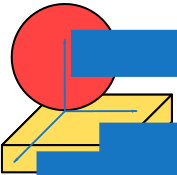
\includegraphics[width=0.8\textwidth]{graphics/friction.pdf} \\
			Wektory tarcia w symulatorach fizyki.\footnotemark
			\column{0.5\textwidth}
			\centering
			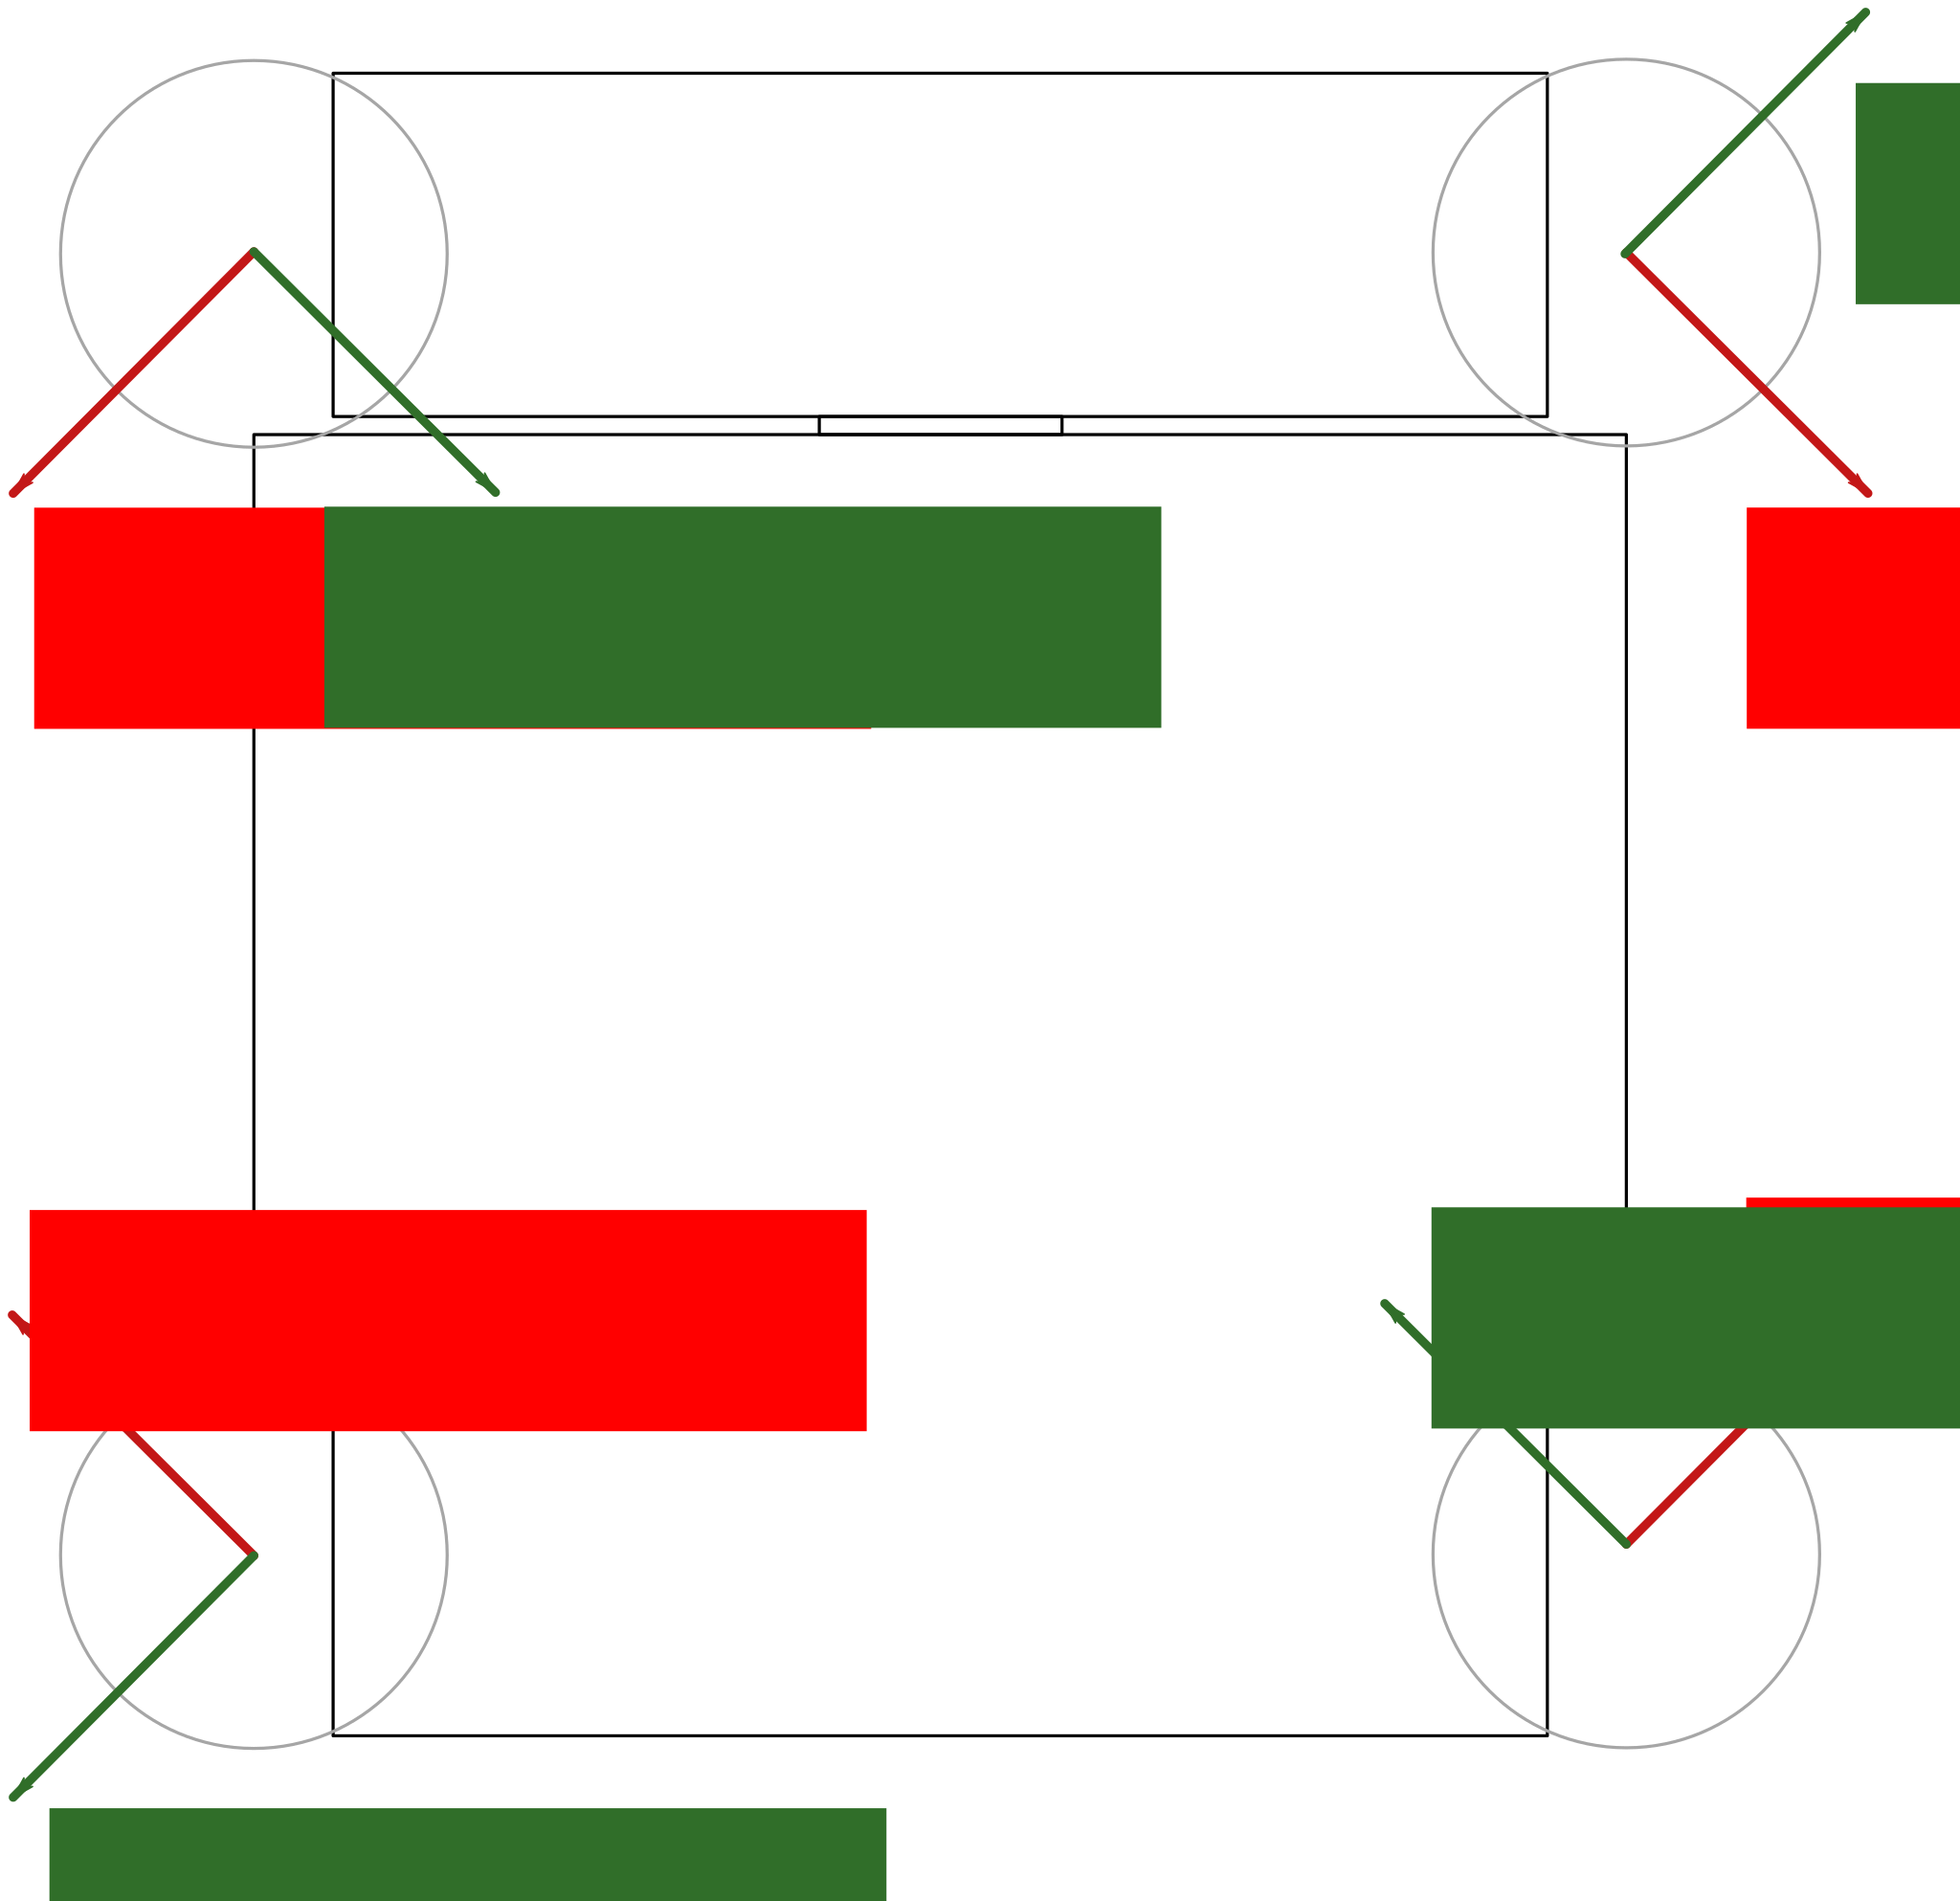
\includegraphics[width=0.8\textwidth]{graphics/base_vects.pdf} \\
			Ustawienie wektorów tarcia w modelu. Ruch w kierunku F1 jest ograniczony, w F2 nieograniczony.
		\end{columns}
		\footnotetext{Na podstawie obrazka z dokumentacji ODE: http://www.ode-wiki.org/wiki/index.php?title=Manual:\_Joint\_Types\_and\_Functions}
	\end{frame}
	
	\section{Komunikacja}
	\begin{frame}
		\frametitle{Wszystkie składowe}
		\begin{description}
			\item[Omnivelma] Model dynamiczny reagujący na siły.
			\item[Pseudovelma] Model kinematyczny, sterowany wzorem.
			\item[Velmaverse] Skrypt uruchamiający Gazebo z definicją symulacji.
			\item[Transmutator] Program tłumaczący zadany ruch na prędkości kół.
			\item[Ocznica] Skrypt obserwujący scenę i produkujący informacje.
			\item[Flooria] Podłoże ze zmiennym współczynnikiem tarcia.
		\end{description}
	\end{frame}
	\begin{frame}
		\frametitle{Komunikacja wewnętrzna i zewnętrzna}
		\centering
		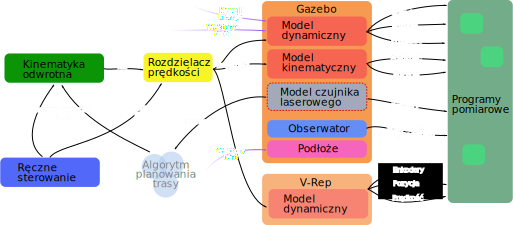
\includegraphics[width=\textwidth]{graphics/comm.pdf}
	\end{frame}
	
	\section{Problemy}
	\begin{frame}
		\frametitle{Największe przeszkody w trakcie tworzenia}
		\begin{enumerate}
			\item Nieodpowiednie ustawienie zależności w \texttt{CMakeLists.txt}.
			\item Niezaimplementowane, a udokumentowane funkcjonalności.
			\item Niewystarczająco dokładnie opisane API.
			\item Niewielkie zainteresowanie tematem na forach i martwe linki.
			\item Nieprzewidywalne zachowanie maszyny symulacyjnej.
			\item Brak wsparcia twórców podobnych modeli.
			\item Zależności od dokładnych wersji bibliotek i niemożność uruchomienia na nie-Ubuntu.
		\end{enumerate}
	\end{frame}
 
	\section{Przyszłość}
	\begin{frame}
		\frametitle{Ku przyszłości}
		\begin{itemize}
			\item Moduł do łatwego sterowania z klawiatury, lub kontrolera.
			\item Ustawienie odpowiednich współczynników modelu w celu uzyskania zadowalającej jakości symulacji.
			\item Testowanie tego samego sterowania, co w symulacji na rzeczywistym robocie i zebranie wyników.
			\item Implementacja modelu w V-REPie. 
		\end{itemize}
	\end{frame}
\end{document}